\section{Structure and Usage of the Movie Ontology}
Our semantic search webpage should enable a user to search for movies or other associated artifacts, e.g. a particular genre or a film's most famous actors. Thus an ontology is required which puts all of those things in relation. We decided to adopt an existing ontology, called "MO - the Movie Ontology" \cite{bouza:movieontology}. It makes use of OWL to map movie entities to classes and defines class hierarchies as well as predicates that show their relationship. To describe its elements, it uses other well-known ontologies, e.g. from "DBpedia" \cite{dbpedia-swj}. Although the used ontology provides a lot of entities, only a subset of them is used for the webpage. The following sections introduce the entities that can be searched and their associated predicates. For the sake of readability, the prefix of a complete URI is omitted.

\subsection{Movie}
A movie is represented as an OWL class. It is the central element of the ontology. Listing \ref{lst:movie} shows how it is defined in an RDF file that uses RDF/XML notation.

\begin{lstlisting}[caption={OWL Movie Class in RDF/XML notation},label={lst:movie}]
<owl:Class rdf:about="&www;Movie"/>.
\end{lstlisting}

Most of the other parts of the ontology have a direct or indirect connection to it, i.e. a predicate describing their relationship. An example is given in listing \ref{lst:movie-pred}. As a movie usually belongs to one or more genres, this is represented by the predicate belongsToGenre. The range and domain entries define the OWL classes that are used as subject (domain $\rightarrow$ a movie) or object (range $\rightarrow$ a genre) in a statement that uses belongsToGenre as its predicate.

\begin{lstlisting}[caption={Exemplary Movie predicate in RDF/XML notation},label={lst:movie-pred}]
<owl:ObjectProperty rdf:about="&movieontology;belongsToGenre">
        <rdfs:range rdf:resource="&movieontology;Genre"/>
        <rdfs:domain rdf:resource="&www;Movie"/>
    </owl:ObjectProperty>
\end{lstlisting}

\subsection{Actor}
Another important part of the ontology is the OWL class for actors, shown in listing \ref{lst:actor}. It is a base class of Person, which itself is part of DBpedia's ontology. That means every Actor implicitly must be a Person and inherits the properties of a Person, too.

\begin{lstlisting}[caption={OWL Actor Class in RDF/XML notation},label={lst:actor}]
<owl:Class rdf:about="&ontology;Actor">
	<rdfs:subClassOf rdf:resource="&ontology;Person"/>
</owl:Class>
\end{lstlisting}

An actor or actress plays in a movie. This is what the predicate in listing \ref{lst:actor-pred} is about. It defines the relationship hasActor between a Movie and an Actor and its reverse definition:
\begin{itemize}
	\item Movie hasActor Actor.
	\item Actor isActorIn Movie.
\end{itemize}

\begin{lstlisting}[caption={Exemplary Actor predicate in RDF/XML notation},label={lst:actor-pred}]
<owl:ObjectProperty rdf:about="&movieontology;hasActor">
	<rdfs:range rdf:resource="&ontology;Actor"/>
	<owl:inverseOf rdf:resource="&movieontology;isActorIn"/>
	<rdfs:domain rdf:resource="&www;Movie"/>
</owl:ObjectProperty>
\end{lstlisting}

\begin{figure}[h]
	\centering
	\fbox{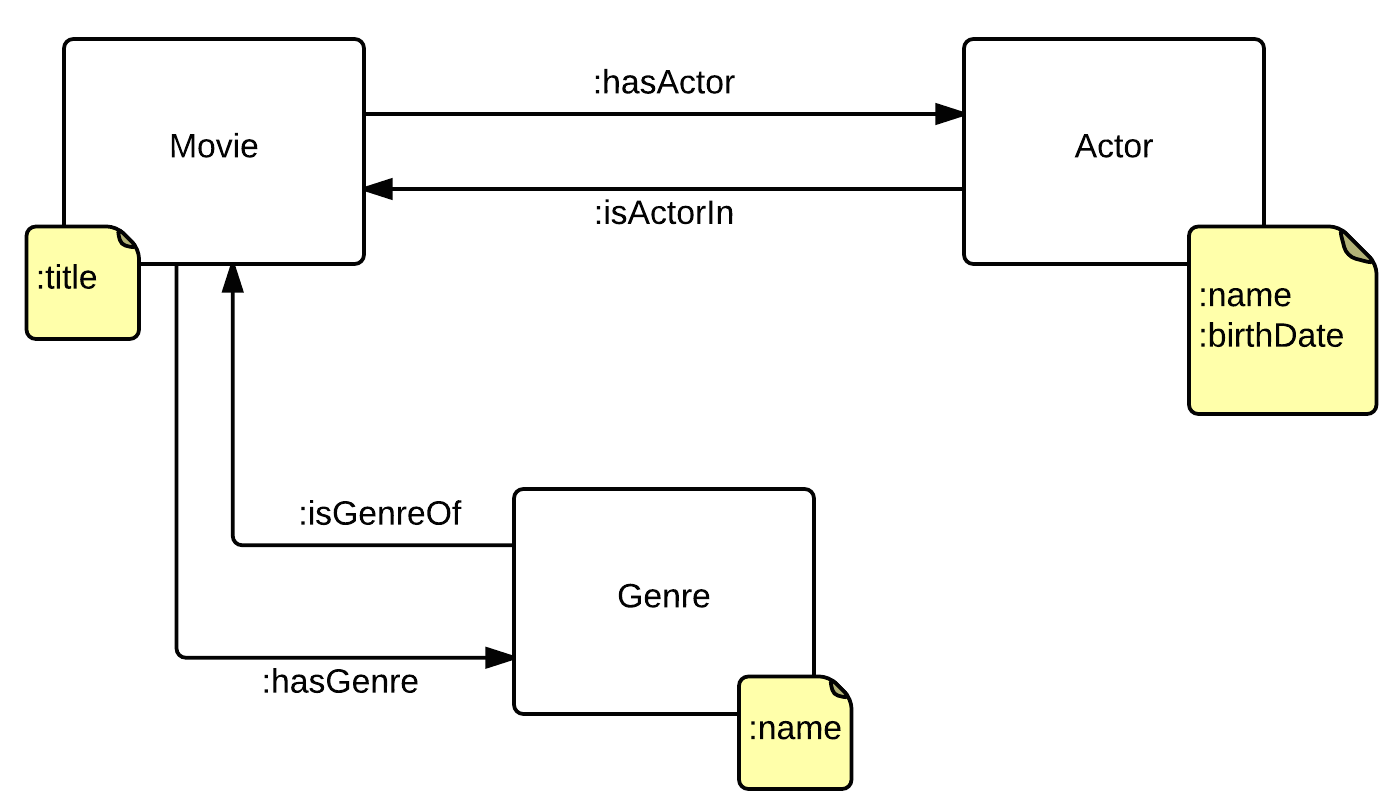
\includegraphics[width=0.8\textwidth]{res/movie-ont.png}}
	\caption{Movie Ontology Overview}
	\label{fig:movie-ont}
\end{figure}

